\documentclass{beamer}
%\documentclass[notes]{beamer}

\usepackage{hyperref}
\usepackage{url}
\usepackage{Sweave}
\usepackage{subfigure}
%\usepackage[utf8]{inputenc}
%\usepackage{booktabs}
\usepackage{caption}
\usepackage{float} 
\usepackage{attrib} 
\usepackage{xcolor} 
%\usepackage{multicol}
\usepackage{tikz}
\usepackage{graphicx}
\usepackage{transparent}
\usetikzlibrary{shapes,backgrounds}
\usetikzlibrary{automata}
\usetikzlibrary{arrows,positioning}
\usetikzlibrary{trees}
\usepackage{tikz-qtree}
%\usetikzlibrary{bayesnet}

%\usepackage{signalflowdiagram}

\usepackage{listings}
\lstset{
language=Python,
basicstyle=\ttfamily,
columns=fullflexible
}

\usepackage{schemabloc}
\usepackage[framemethod=tikz]{mdframed}

\definecolor{links}{HTML}{2A1B81}
\hypersetup{colorlinks,linkcolor=,urlcolor=links}

\definecolor{mydarkblue}{HTML}{0066CC}
\definecolor{mydarkred}{HTML}{990000}
\definecolor{mydarkgreen}{HTML}{006600}
\definecolor{myblue}{HTML}{336699}

\tikzstyle{normalnode}=[draw,%
                          rectangle,%
                          shade,%
                          minimum size  = 1.0cm,%
                          node distance = 1.3cm]
 \tikzstyle{normalnode2}=[draw,%
                          rectangle,%
                          shade,%
                          minimum size  = 1.0cm,%
                          node distance = 1.0cm]
  \tikzstyle{normalnode3}=[draw,%
                          rectangle,%
                          shade,%
                          minimum size  = 1.0cm,%
                          node distance = 5.0cm]
  \tikzstyle{normal}=[draw,fill=myblue,rectangle, minimum size=1.0cm,node
  distance=2cm, text=white] 
  \tikzstyle{start}=[draw,fill=green!70,rectangle, minimum size=1.0cm,node distance=1.3cm]                        
  \tikzstyle{goal}=[draw,fill=red!70,rectangle, minimum size=1.0cm,node distance=1.3cm]
  \tikzstyle{goal2}=[draw,fill=red!70,rectangle, minimum size=1.0cm,node distance=1.0cm]
  \tikzstyle{agent}=[draw,fill=blue!70,circle,minimum size=0.6cm]
  \tikzstyle{dummy}=[circle]
\usetikzlibrary{automata,chains}

\usetikzlibrary{positioning}
\usetikzlibrary{intersections}

\definecolor{myblue}{HTML}{336699}

\setbeamertemplate{blocks}[rounded=true, shadow=true] 
\setbeamercolor{block title}{bg=myblue,fg=white}
\setbeamercolor{frametitle}{myblue}
\setbeamercolor{title}{myblue}
\usecolortheme[named=myblue]{structure}

%% Add support for \subsubsectionpage
%\def\subsubsectionname{\translate{Subsubsection}}
%\def\insertsubsubsectionnumber{\arabic{subsubsection}}
%\setbeamertemplate{section page}
%{
%  \begin{centering}
%    \begin{beamercolorbox}[sep=4pt,center]{part title}
%      \usebeamerfont{section title}\insertsection\par
%    \end{beamercolorbox}
%  \end{centering}
%}
%\setbeamertemplate{subsubsection page}
%{
%  \begin{centering}
%    {\usebeamerfont{subsubsection name}\usebeamercolor[fg]{subsubsection
%    name}\subsubsectionname~\insertsubsubsectionnumber} 
%    \vskip1em\par
%    \begin{beamercolorbox}[sep=4pt,center]{part title}
%      \usebeamerfont{subsubsection title}\insertsubsubsection\par
%    \end{beamercolorbox}
%  \end{centering}
%}
%\def\subsubsectionpage{\usebeamertemplate*{subsubsection page}}
%
%\AtBeginSection{\frame{\sectionpage}}
%\AtBeginSubsection{\frame{\subsectionpage}}

\begin{document}
\Sconcordance{concordance:ai_sota.tex:ai_sota.Rnw:%
1 776 1 1 33 1 114 266 1}

\title{The 10,000 Hours Rule} 
\subtitle{Learning to Play Games with AI}
\author{Shane Conway} 
\institute{
%\textit{smc77@columbia.edu, @statalgo} 
}
\date{\today} 

\AtBeginSection[]{
   \setbeamercolor{section in toc shaded}{use=structure,fg=structure.fg}
   \setbeamercolor{section in toc}{fg=myblue}
   \setbeamercolor{subsection in toc shaded}{fg=black}
   \setbeamercolor{subsection in toc}{fg=myblue}
  \frame<beamer>{%\begin{multicols}
  \frametitle{Outline}
  \setcounter{tocdepth}{2}  
  \tableofcontents[currentsection,subsections]
%\end{multicols} 
 }
}


{
  \usebackgroundtemplate{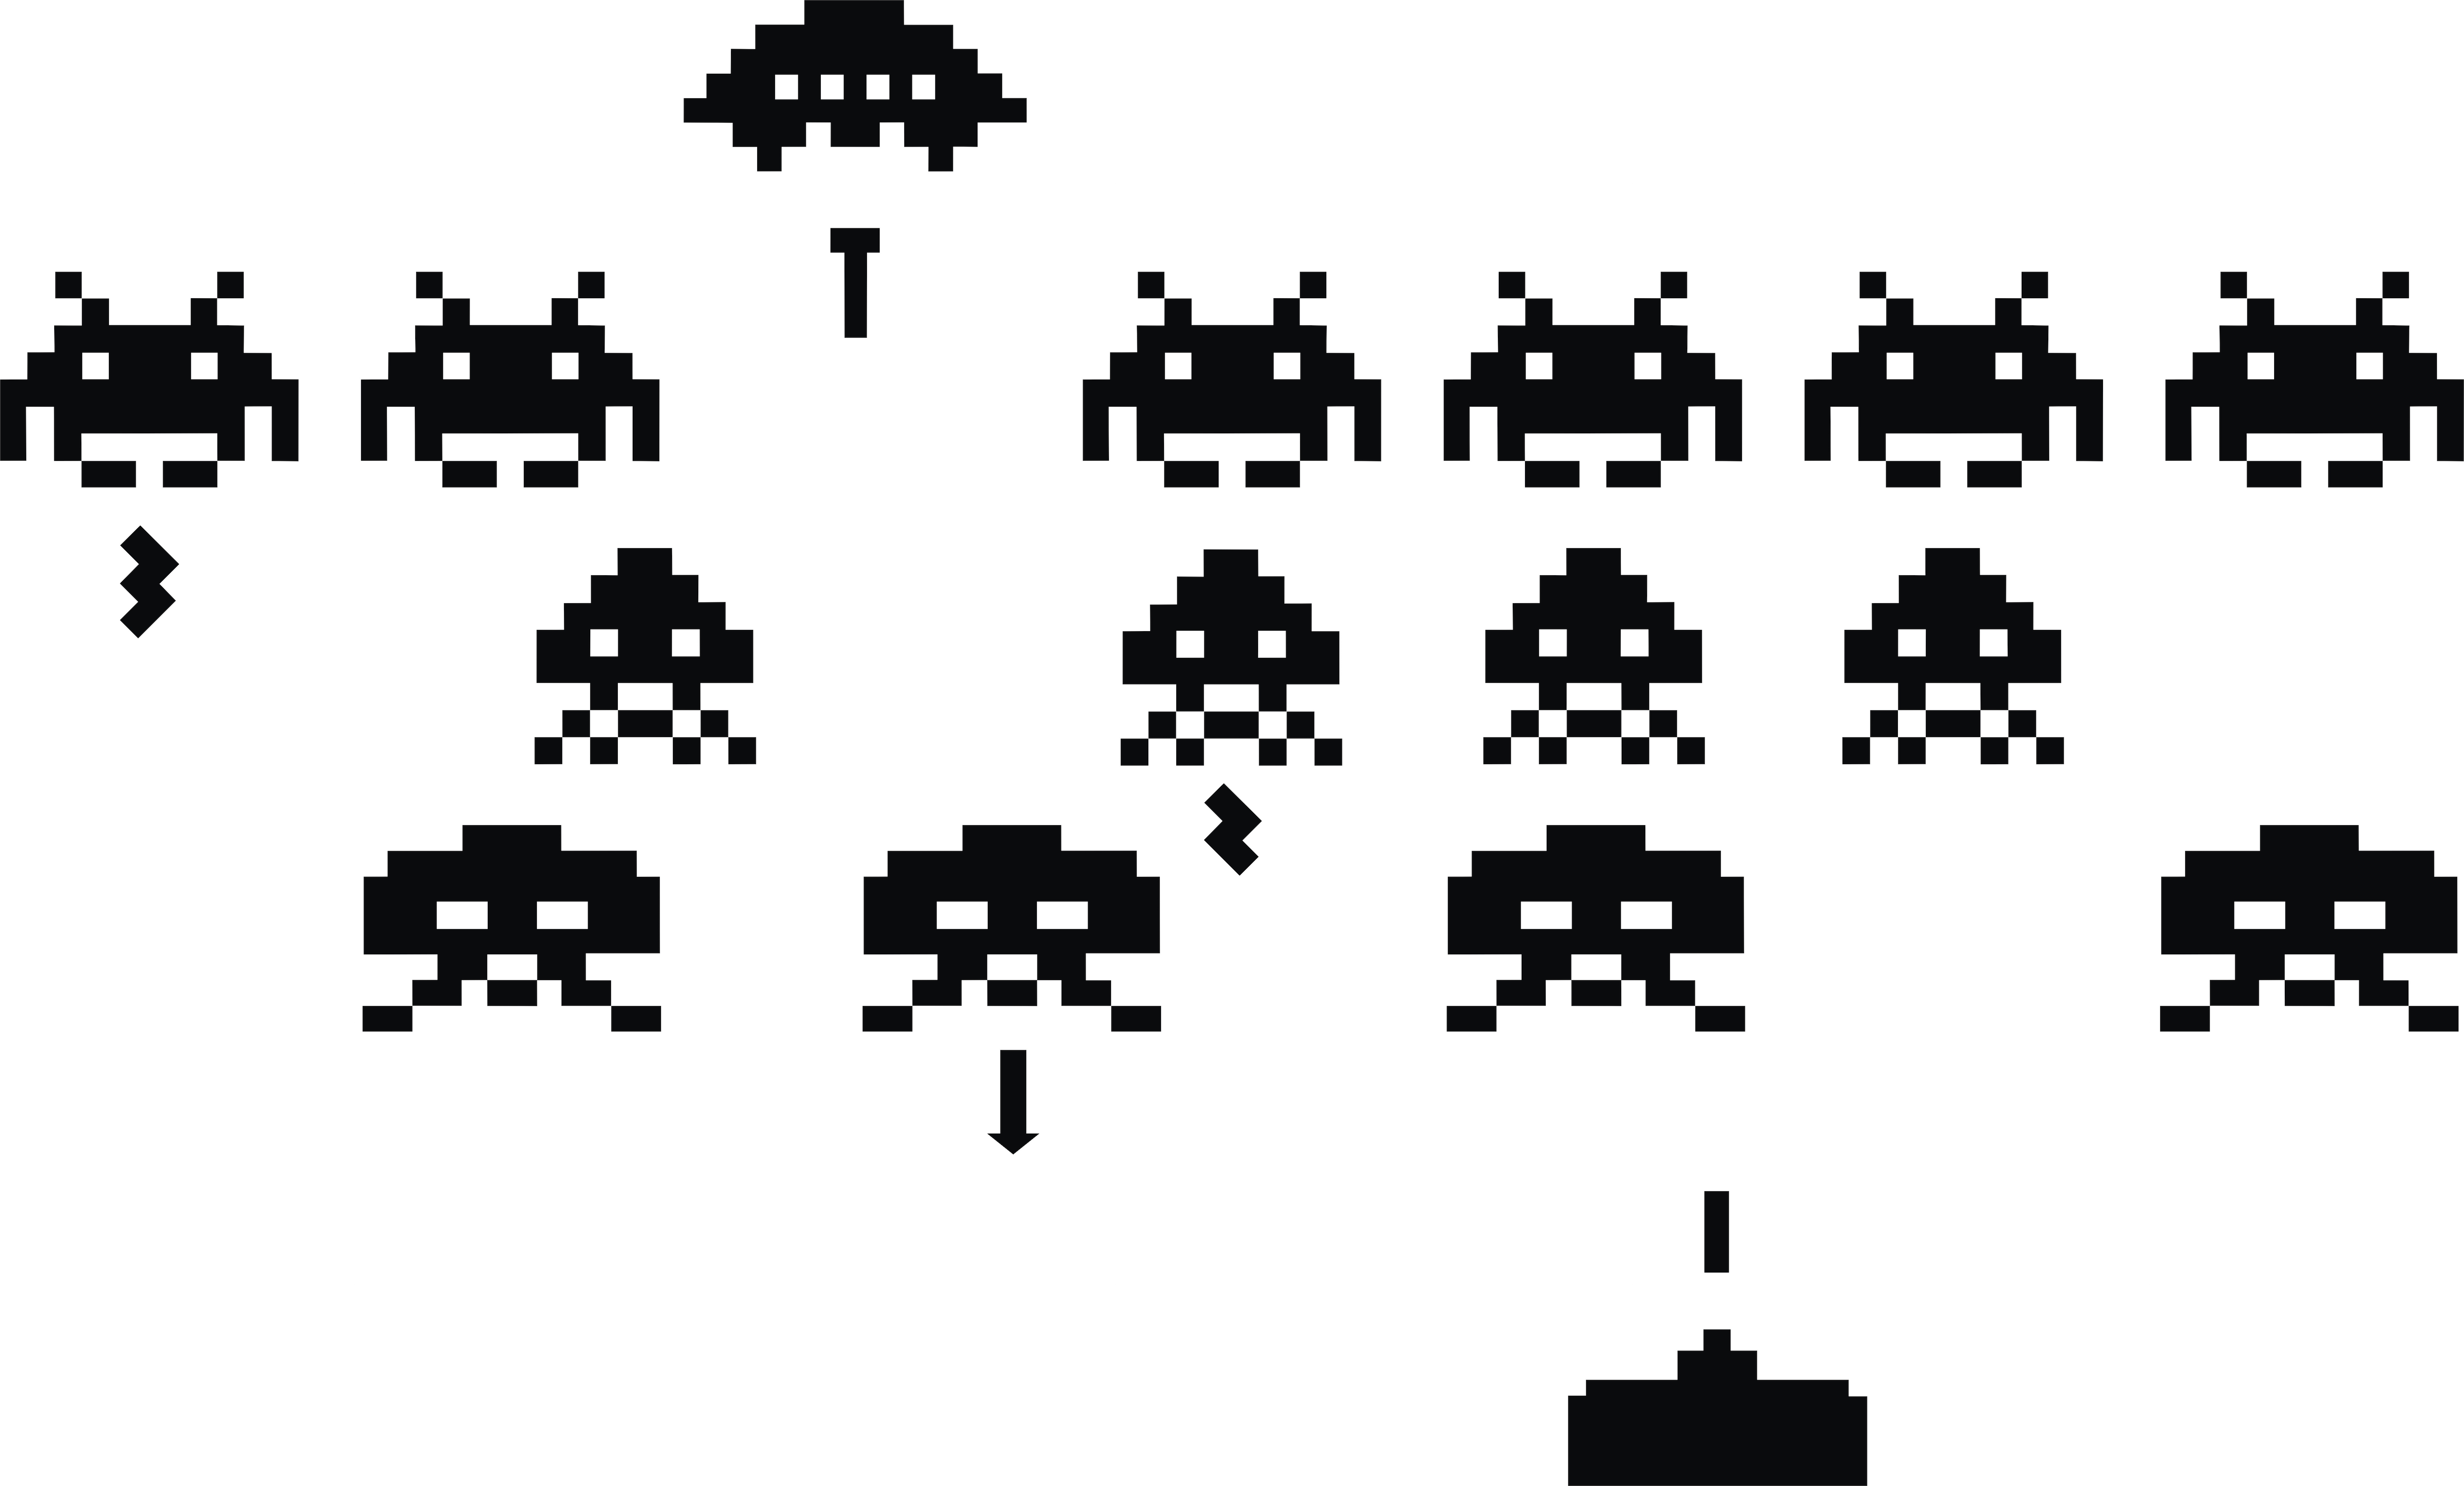
\includegraphics[width=1.0\paperwidth, height=1.0\paperheight]{figures/spaceinvaders.png}} %
  \begin{frame}[plain]
\vspace{15em}
\begin{mdframed}[tikzsetting={draw=black,fill=white,fill opacity=0.7,
               line width=4pt},backgroundcolor=none,leftmargin=0,
               rightmargin=40,innertopmargin=4pt]
{\huge State of the Art in AI}\\
A Short Introduction\\
Shane M. Conway, Kepos Capital\\
\end{mdframed}
  \end{frame}
}

% \frame{\titlepage} 



\frame{

\begin{quote}
"I think we should be very careful about artificial intelligence. If I had to guess at what our biggest existential threat is, it's probably that. So we need to be very careful.  I'm increasingly inclined to think that there should be some regulatory oversight, maybe at the national and international level, just to make sure that we don't do something very foolish." -Elon Musk
\end{quote}

\note{
}

%\pause

% \begin{quote}
% "The use of punishments and rewards can at best be a part of the teaching process. Roughly speaking, if the teacher has no other means of communicating to the pupil, the amount of information which can reach him does not exceed \textbf{the total number of rewards and punishments applied}." \href{http://orium.pw/paper/turingai.pdf
% }{(Turing (1950) "Computing Machinery and Intelligence")}
% \end{quote}
% 
% \note{
% Alan Turing famously considered the ideas of reinforcement learning when developing his ideas around the measures of AI (the Turing Test).
% \begin{itemize}
% \item "the total number of rewards and punishments applied": there is some function that accumulates knowledge of rewards and punishments, which is the value function in RL.
% \end{itemize}
% }

}

\frame{\frametitle{Outline}\tableofcontents} 

% Resources:
% http://users.isr.ist.utl.pt/~mtjspaan/readingGroup/slides04012007.pdf


\section{What is AI?} 

{
\usebackgroundtemplate{% width=\paperwidth,
\parbox[c][\paperheight][c]{\paperwidth}{
\begin{figure}[H]
\begin{center}
%   \tikz\node[opacity=0.2] {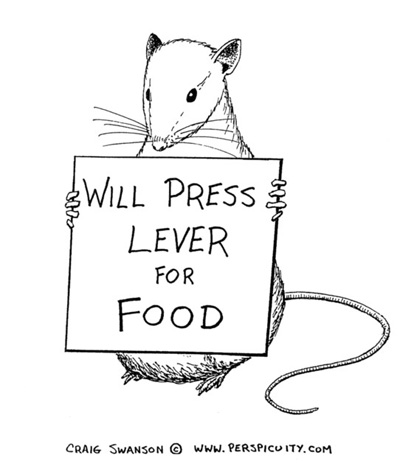
\includegraphics[height=\paperheight, right]{../images/cartoon_4.jpg}};
\end{center}
\end{figure}
}
}

\frame{

\begin{center}
{\huge Artificial Intelligence}\\

\vspace{12 mm}

\pause

{\Large What is it and why should we care?}
\end{center}

}
}


\frame{%\frametitle{Twitter Crash} 

\begin{figure}[!h]
\begin{center}
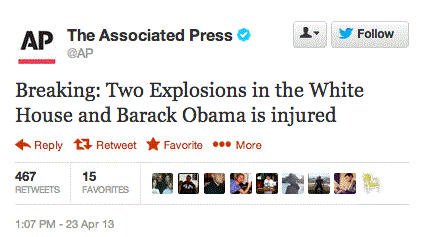
\includegraphics[width=0.9\textwidth]{figures/fake-ap-tweet.png}
\end{center}
%\caption{AI has a long history.}
\end{figure}

%\scriptsize{\textit{\href{http://247wallst.com/investing/2013/04/23/a-new-mini-flash-crash-from-fake-ap-tweet-hack-attack/}{"A New Mini Flash Crash from Fake AP Tweet, Twitter Hack Attack" Bloomberg (2013)}}}

}

\frame{\frametitle{Twitter Crash} 

\begin{figure}[!h]
\begin{center}
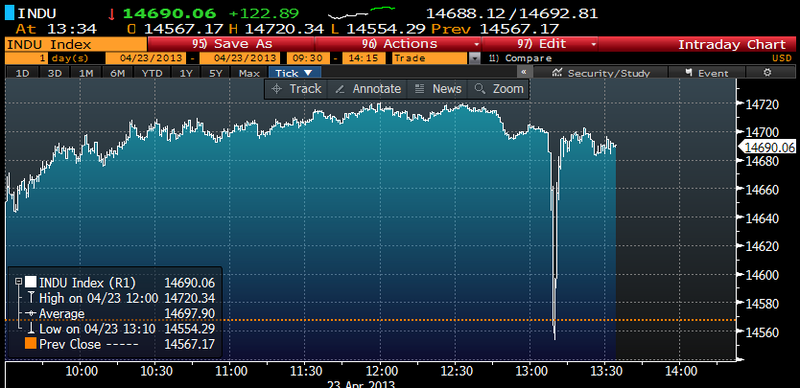
\includegraphics[width=1\textwidth]{figures/twitter_crash.png}
\end{center}
%\caption{AI has a long history.}
\end{figure}

\scriptsize{\textit{\href{https://www.bloomberg.com/news/articles/2013-04-23/a-fake-ap-tweet-sinks-the-dow-for-an-instant}{"A Fake AP Tweet Sinks the Dow for an Instant" Bloomberg (2013)}}}

}



\frame{\frametitle{Trends} 


\begin{figure}[!h]
\begin{center}
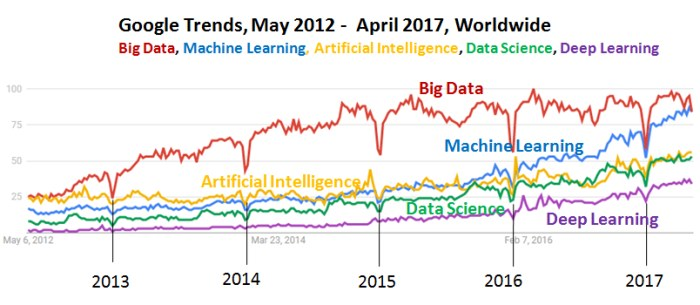
\includegraphics[width=1\textwidth]{figures/google_trends.jpg}
\end{center}
%\caption{AI has a long history.}
\end{figure}

\scriptsize{\textit{\href{https://trends.google.com/trends/explore?date=all&q=Machine%20Learning,Big%20Data,Artificial%20Intelligence,Data%20Science,Deep%20Learning
}{Source: Google Trends}}}

}


\frame{\frametitle{Artificial Intelligence} 

\begin{figure}[!h]
\begin{center}
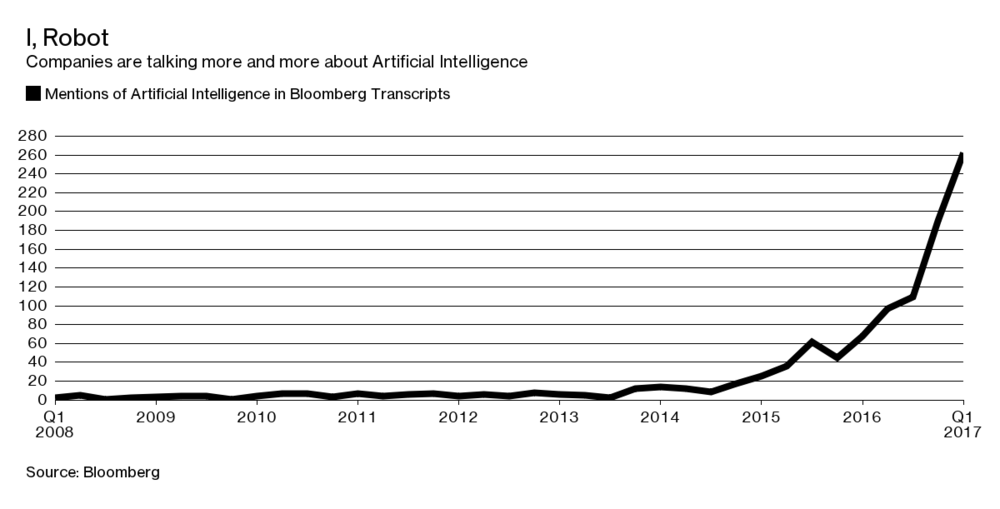
\includegraphics[width=1\textwidth]{figures/Eco-11.png}
\end{center}
%\caption{AI has a long history.}
\end{figure}

\scriptsize{\textit{\href{https://www.bloomberg.com/news/articles/2017-06-13/the-limits-of-artificial-intelligence}{"The Limits of Artificial Intelligence" Bloomberg (June 2017)}}}


}
% 
% \frame{\frametitle{Hedge Funds} 
% 
% 
% 
% }
% 


\frame{\frametitle{This isn't new...} 

\begin{figure}[!h]
\begin{center}
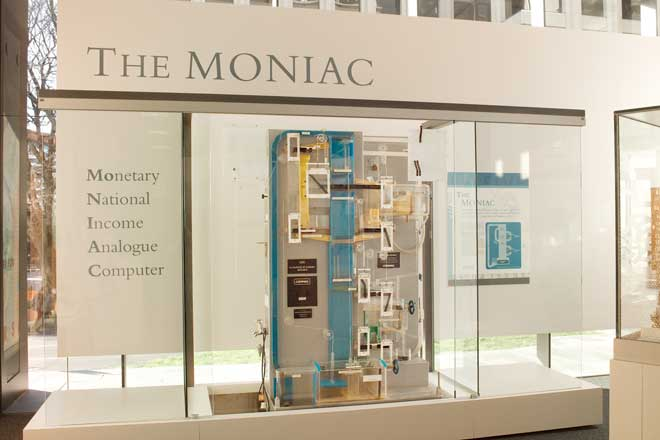
\includegraphics[width=0.8\textwidth]{figures/moniac.jpg}
\end{center}
%\caption{AI has a long history.}
\end{figure}

\vspace{0.10in}

\scriptsize{\textit{\href{https://en.wikipedia.org/wiki/MONIAC}{MONIAC (Monetary National Income Analogue Computer) Bill Phillips (1949)}}}

}



\frame{\frametitle{History of AI} 

\begin{figure}[!h]
\begin{center}
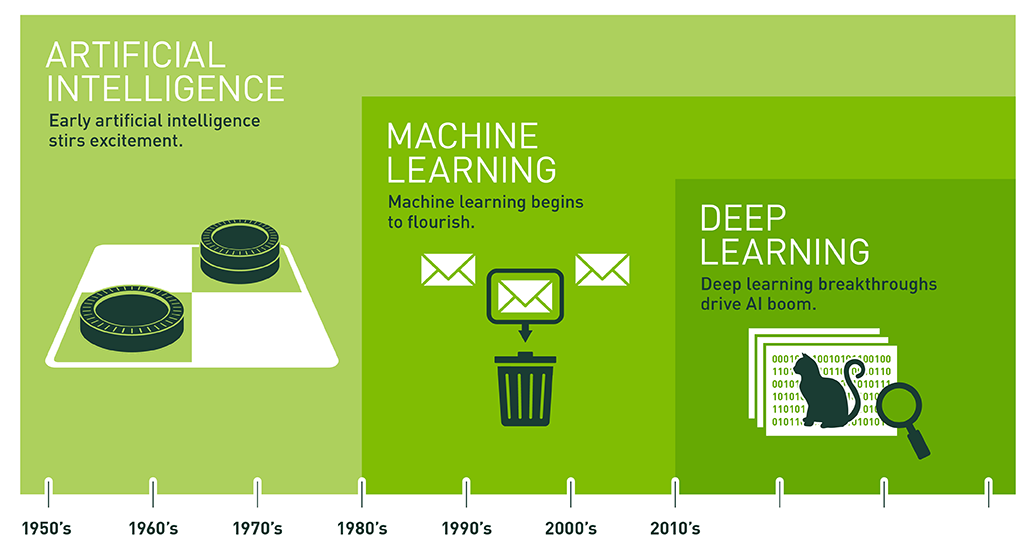
\includegraphics[width=1\textwidth]{figures/Deep_Learning_History.png}
\end{center}
%\caption{AI has a long history.}
\end{figure}

\vspace{0.25in}

\scriptsize{\textit{\href{https://blogs.nvidia.com/blog/2016/07/29/whats-difference-artificial-intelligence-machine-learning-deep-learning-ai/}{Image source: nvidia}}}


}



\frame{\frametitle{Artificial Intelligence: Why now?} 

\begin{enumerate}
  \item Compute (the obvious one: Moore's Law, GPUs, ASICs),
  \item Data (in a nice form, not just out there somewhere on the internet - e.g. ImageNet),
  \item Algorithms (research and ideas, e.g. backprop, CNN, LSTM), and
  \item Infrastructure (software under you - Linux, TCP/IP, Git, ROS, PR2, AWS, AMT, TensorFlow, etc.).
\end{enumerate}


\vspace{0.25in}

\scriptsize{\textit{\href{http://karpathy.github.io/2016/05/31/rl/}{Source: @karpathy}}}
% 

}


\frame{\frametitle{Artificial} 

AI is an \emph{artificial} (as opposed to \emph{natural}) science:

\begin{enumerate}
  \item Artificial things are synthesized by human beings.
  \item Artificial things may imitate appearances of natural things while lacking the reality of the latter.
  \item Artificial things can be characterized in terms of functions, goals, adaptation.
  \item Artificial things are often discussed in terms of imperatives as well as descriptives.
\end{enumerate}


\vspace{0.25in}

\scriptsize{\textit{\href{https://mitpress.mit.edu/books/sciences-artificial}{Source: Herbert A. Simon "The Sciences of the Artificial" (1968)}}}

}


\frame{\frametitle{Intelligence} 

AI is a form of \emph{intelligence}, in the same sense that human's have intelligence.  Intelligence is hard to define, but "we know it when we see it".

\vspace{0.10in}

Turing formulated the "Imitation Game" (or the turing test).

\vspace{0.10in}

\begin{figure}[!h]
\begin{center}
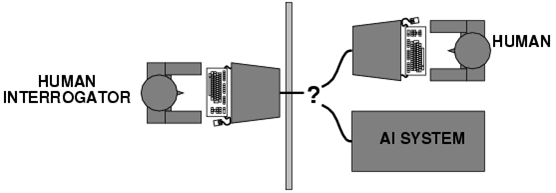
\includegraphics[width=0.8\textwidth]{figures/turing.png}
\end{center}
%\caption{AI has a long history.}
\end{figure}

\vspace{0.10in}

\scriptsize{\textit{\href{https://mitpress.mit.edu/books/sciences-artificial}{Source: Alan Turing "Computing machinery and intelligence" (1950)}}}

}



\frame{\frametitle{Human Intelligence} 

\begin{figure}[!h]
\begin{center}
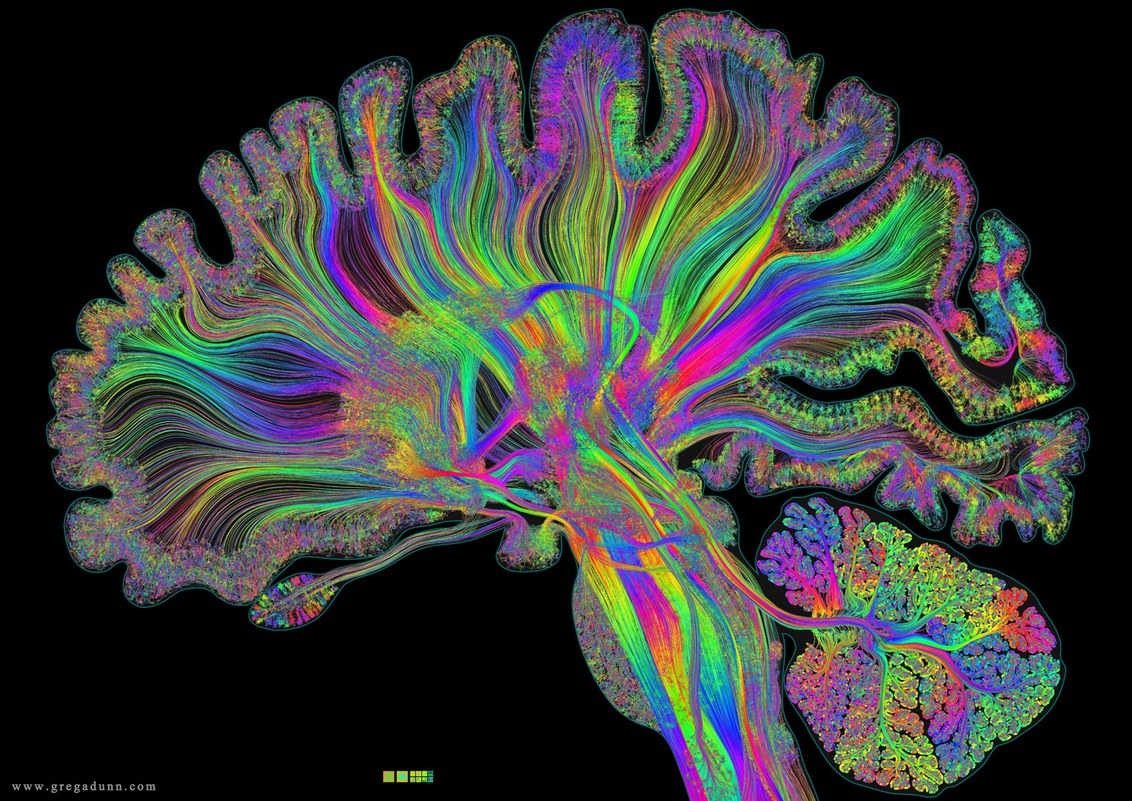
\includegraphics[width=0.9\textwidth]{figures/brain.jpg}
\end{center}
%\caption{AI has a long history.}
\end{figure}

\vspace{0.10in}

\scriptsize{\textit{\href{http://www.gregadunn.com/}{Source: Greg Dunn "Self Reflected"}}}


}



\frame{\frametitle{Human's vs Chimps} 

Human's are "social learners".

\vspace{0.25in}

The big difference between baby humans and chimpanzees is not in mastering abstract ideas, like quantity or causality, but that we are "prolific, spontaneous and automatic imitators, even willing to copy seemingly unnecessary or purely stylistic steps". Under pressure to keep up with culture, we are built to imitate and fit in.

\vspace{0.25in}

\scriptsize{\textit{\href{https://www.newscientist.com/article/mg22830511-100-time-to-rethink-what-makes-humans-special/}{Source: Joseph Henrich "The Secret of Our Success" (2016)}}}

}


\frame{\frametitle{Artificial Intelligence} 

\begin{itemize}
  \item AI involves machines that can perform tasks that are characteristic of human intelligence. (John McCarthy 1956)
  \item ML is a subfield of computer science that "gives computers the ability to learn without being explicitly programmed". (Arthur Samuel, 1959)
\end{itemize}

\begin{figure}[!h]
\begin{center}
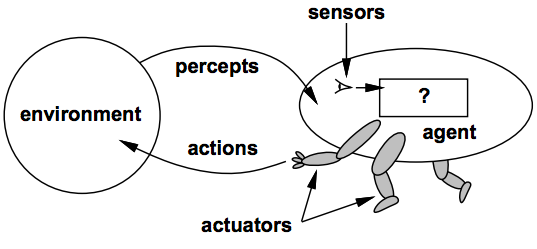
\includegraphics[width=0.6\textwidth]{figures/AIMA.png}
\end{center}
%\caption{AI has a long history.}
\end{figure}

Goal: Construct a single universal agent that learns to act optimally in any environment.

%http://www.hutter1.net/ai/sintro2ai.pdf

}


% \frame{\frametitle{Caveates} 
% 
% I will be discussing the SOTA in AI, and hence will be mostly ignoring:
% 
% \begin{itemize}
%   \item Problems with "small data"
%   \item Theory
%   \item Specific applications within finance
% \end{itemize}
% 
% }
% 



\section{Cutting Edge Applications} 

{
\usebackgroundtemplate{% width=\paperwidth,
\parbox[c][\paperheight][c]{\paperwidth}{
\begin{figure}[H]
\begin{center}
%   \tikz\node[opacity=0.2] {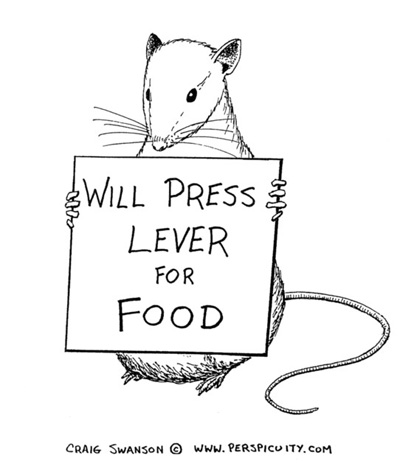
\includegraphics[height=\paperheight, right]{../images/cartoon_4.jpg}};
\end{center}
\end{figure}
}
}

\frame{

\begin{center}
{\huge The State of the Art (SOTA)}\\

\vspace{12 mm}

%\pause

{\Large }
\end{center}

}
}



\frame{\frametitle{Mastering Atari} 

\begin{figure}[!h]
\begin{center}
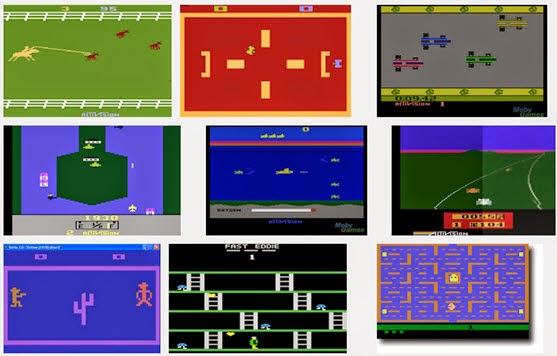
\includegraphics[width=0.98\textwidth]{figures/atari-2600-games.jpg}
\end{center}
\end{figure}

%https://ocr.space/blog/2015/02/playing-atari-deep-reinforcement-learning.html

}


\frame{\frametitle{AlphaGo} 

\begin{figure}[!h]
\begin{center}
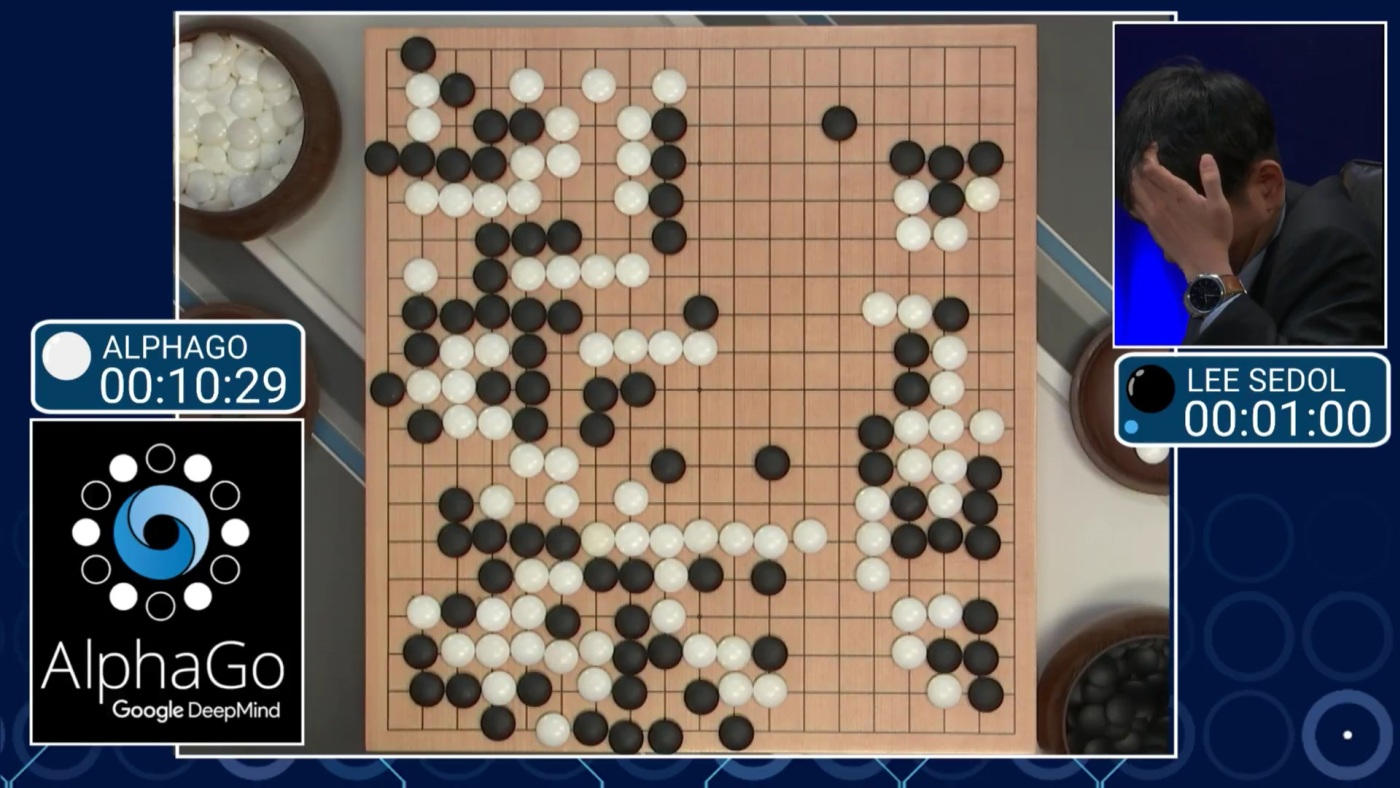
\includegraphics[width=0.98\textwidth]{figures/alphago.jpg}
\end{center}
\end{figure}

\emph{The number of potential legal board positions in go is greater than the number of atoms in the universe.}
%https://www.theatlantic.com/technology/archive/2016/03/the-invisible-opponent/475611/

}



% 
% \frame{\frametitle{Self-Driving Cars} 
% 
% 
% 
% 
% }
% 



\frame{\frametitle{Artwork} 

\begin{figure}[!h]
\begin{center}
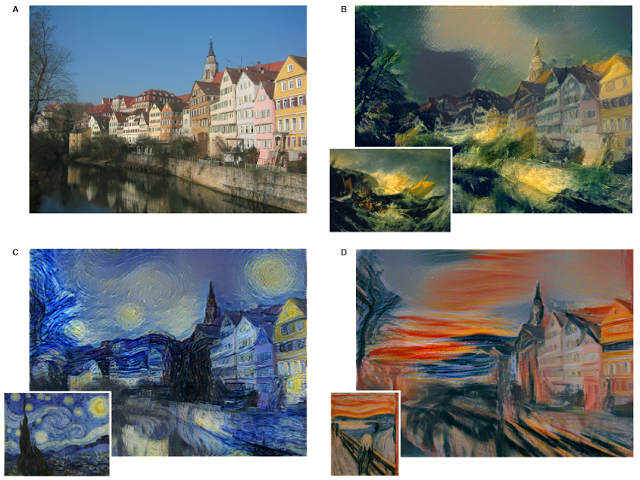
\includegraphics[width=0.9\textwidth]{figures/art.png}
\end{center}
\end{figure}

\scriptsize{\textit{\href{https://arxiv.org/abs/1508.06576}{Source: L. Gatys e. al “A Neural Algorithm of Artistic Style” (2015).}}}

% https://medium.com/udacity/deep-learning-nanodegree-foundation-program-syllabus-in-depth-2eb19d014533

}

% 
% \frame{\frametitle{Speech} 
% 
% DeepMind released WaveNet
% 
% %https://www.slideshare.net/LuMa921/deep-learning-the-past-present-and-future-of-artificial-intelligence
% 
% }



% \frame{\frametitle{Natural Language} 
% 
% 
% 
% }


\frame{\frametitle{Writing Code} 

\begin{figure}[!h]
\begin{center}
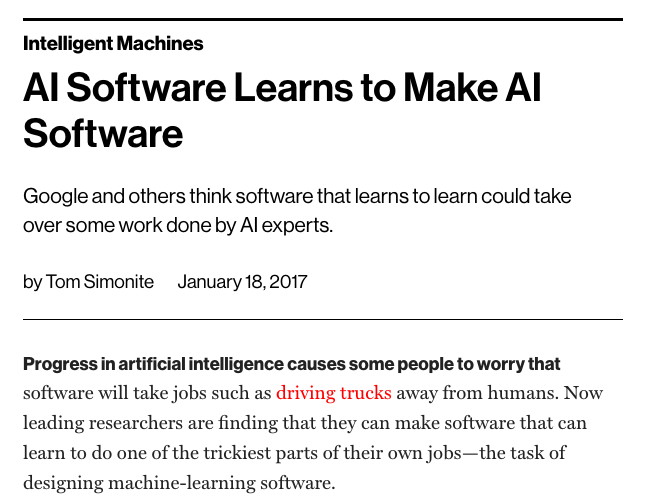
\includegraphics[width=0.9\textwidth]{figures/writing_code.png}
\end{center}
\end{figure}

\scriptsize{\textit{\href{https://www.technologyreview.com/s/603381/ai-software-learns-to-make-ai-software/}{"AI Software Learns to Make AI Software" MIT Technology Review (Jan 2017)}}}

}


% \frame{\frametitle{Robots} 
% 
% 
% 
% }


\frame{\frametitle{Other Examples}

There are many other examples of recent successes:

\begin{itemize}
  \item Self driving cars
  \item Speech (e.g. WaveNet)
  \item Machine translation
  \item Natural language
  \item Image, video classification
  \item Journalism, poetry
  \item Robotics
\end{itemize}


}


\section{Machine Learning} 

{
\usebackgroundtemplate{% width=\paperwidth,
\parbox[c][\paperheight][c]{\paperwidth}{
\begin{figure}[H]
\begin{center}
%   \tikz\node[opacity=0.2] {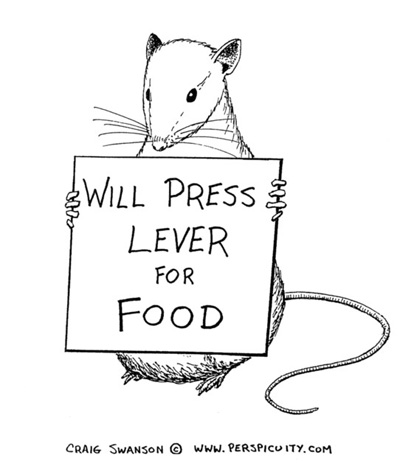
\includegraphics[height=\paperheight, right]{../images/cartoon_4.jpg}};
\end{center}
\end{figure}
}
}

\frame{

\begin{center}
{\huge Machine Learning}\\

\vspace{12 mm}

{\Large Data in...predictions out.}
\end{center}

}
}



%%%%%%%%%%%%%%%%%%%%%%%%%%
\begin{frame}


\begin{figure}
\begin{tikzpicture}[
node distance = 4mm and 22mm
                        ]
\node (adc) [draw,minimum size=24mm] {Model};
%
\coordinate[above left = of adc.west]   (a1);
\coordinate[below = of a1]              (a2);
\coordinate[below = of a2]              (a3);
\coordinate[above right= 8mm and 22mm of adc.east]  (b1);
\foreach \i [count=\xi from 1] in {2,...,5} 
    \coordinate[below=of b\xi]  (b\i);
%
\foreach \i [count=\xi from 1] in {$X_1$, $X_2$, $\dots$}
\draw[-latex']  (a\xi) node[left] {\i} -- (a\xi-| adc.west);
\foreach \i [count=\xi from 3] in {Y}
    \draw[-latex'] (adc.east |- b\xi) -- (b\xi) node[right] {\i};
\end{tikzpicture}
\end{figure}

\end{frame}

%%%%%%%%%%%%%%%%%%%%%%%%%%
\begin{frame}
\frametitle{Machine Learning}

Machine learning includes several different kinds of \emph{models}:

%\pause

\vspace{0.25in}

\begin{itemize}
  \item Supervised learning: learn a function by fitting labeled targets and input features.
%\pause
  \item Unsupervised learning: learn a function by fitting to input features (without labeled targets).
%\pause
  \item Reinforcement learning: learn a policy based on receiving rewards for taking actions in states.
\end{itemize}

\end{frame}
%%%%%%%%%%%%%%%%%%%%%%%%%%

\begin{frame}
\frametitle{Models}

There are a wide variety of models that serve different purposes, such as:

\begin{itemize}
  \item Linear regression
  \item Logistic regression
  \item Neural networks
  \item Support vector machines
  \item Random forests
  \item Gradient Boosted Machines
\end{itemize}

\end{frame}
%%%%%%%%%%%%%%%%%%%%%%%%%%

%%%%%%%%%%%%%%%%%%%%%%%%%%
\begin{frame}
\frametitle{Machine Learning Pipeline}

Machine learning in practice is more than \emph{models}; it includes a set of tools to make predictions robust.

%\pause

\vspace{0.25in}

\begin{itemize}
\item Feature engineering
%\pause
\item Regularization
%\pause
\item Feature selection
%\pause
\item Hyperparameter tuning
%\pause
\item Model selection
%\pause
\item Ensembling
\end{itemize}

\end{frame}
%%%%%%%%%%%%%%%%%%%%%%%%%%


\section{Deep Learning} 

{
\usebackgroundtemplate{% width=\paperwidth,
\parbox[c][\paperheight][c]{\paperwidth}{
\begin{figure}[H]
\begin{center}
%   \tikz\node[opacity=0.2] {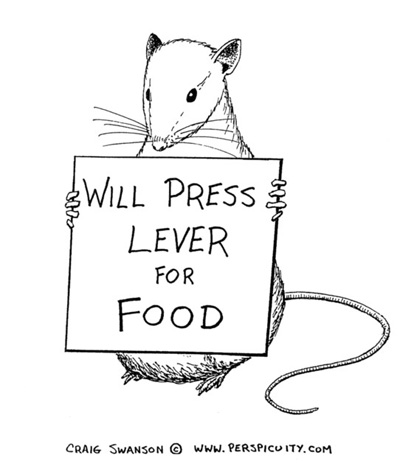
\includegraphics[height=\paperheight, right]{../images/cartoon_4.jpg}};
\end{center}
\end{figure}
}
}

\frame{

\begin{center}
{\huge Deep Learning}\\

\vspace{12 mm}

{\Large Generalizing from what we see.}
\end{center}

}
}



%%%%%%%%%%%%%%%%%%%%%%%%%%
\begin{frame}
\frametitle{Neural Networks} 

\emph{Artificial neural networks} (ANN) are learning models that were directly inspired by the structure of biological neural networks.

\begin{figure}[!h]
\begin{center}
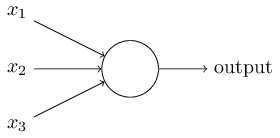
\includegraphics[width=0.45\textwidth]{figures/tikz0.png}
\end{center}
\end{figure}

\begin{eqnarray}
  \mbox{output} & = & \left\{ \begin{array}{ll}
      0 & \mbox{if } \sum_j w_j x_j \leq \mbox{ threshold} \\
      1 & \mbox{if } \sum_j w_j x_j > \mbox{ threshold}
      \end{array} \right.
\tag{1}\end{eqnarray}

%\vspace{0.15in}

%\scriptsize{\textit{\href{https://medium.com/@jaschaephraim/elementary-neural-networks-with-tensorflow-c2593ad3d60b#.hidaox4qi}{Image source: @jaschaephraim}}}
%http://neuralnetworksanddeeplearning.com/chap1.html

%http://cs231n.github.io/neural-networks-1/
%Source: https://medium.com/@jaschaephraim/elementary-neural-networks-with-tensorflow-c2593ad3d60b#.8nuva6y4z
%http://sebastianraschka.com/Articles/2015_singlelayer_neurons.html
%https://stevenmiller888.github.io/mind-how-to-build-a-neural-network/

\end{frame}

%%%%%%%%%%%%%%%%%%%%%%%%%%
\begin{frame}
\frametitle{Multi-layer Neural Networks} 

\begin{figure}[!h]
\begin{center}
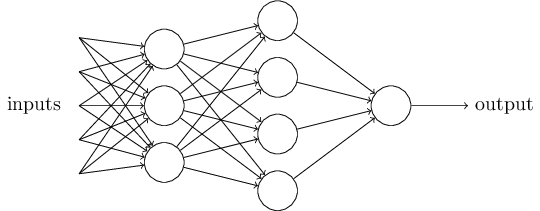
\includegraphics[width=0.8\textwidth]{figures/tikz1.png}
\end{center}
\caption{Multiple layers can be connected together.}
\end{figure}

%http://cs231n.github.io/convolutional-networks/
%https://beckmw.wordpress.com/2013/11/14/visualizing-neural-networks-in-r-update/

\end{frame}

%%%%%%%%%%%%%%%%%%%%%%%%%%
\begin{frame}



Multi-layer neural networks can fit complex functions:

\begin{figure}[h!]
\centering
\begin{minipage}{.5\textwidth}
  \centering
  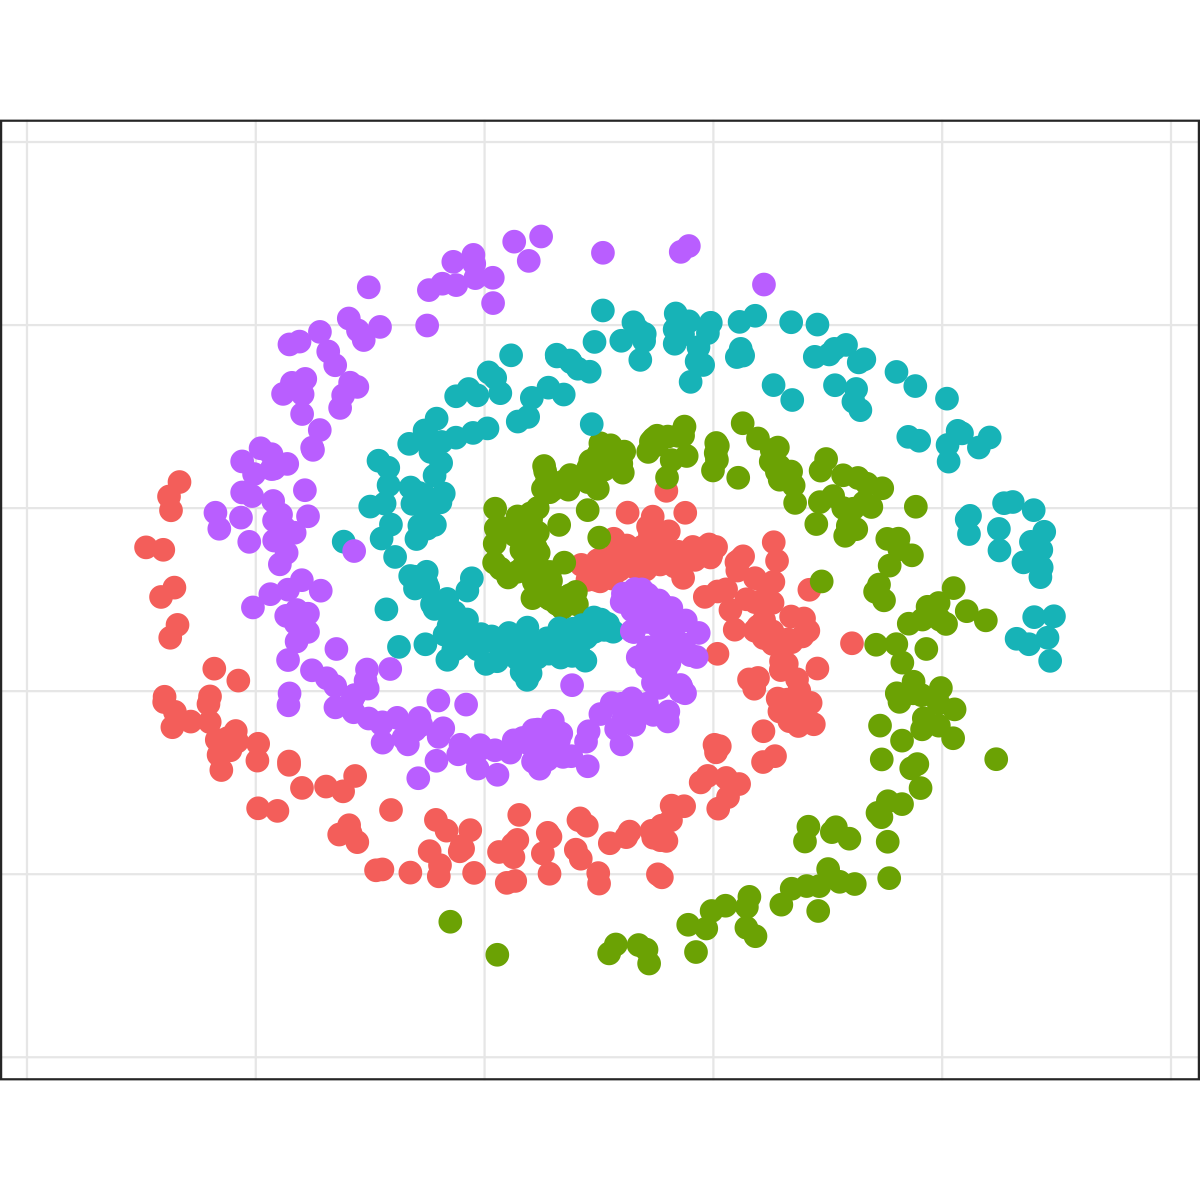
\includegraphics[width=0.9\textwidth]{figures/spiral.png}
\end{minipage}%
\begin{minipage}{.5\textwidth}
  \centering
  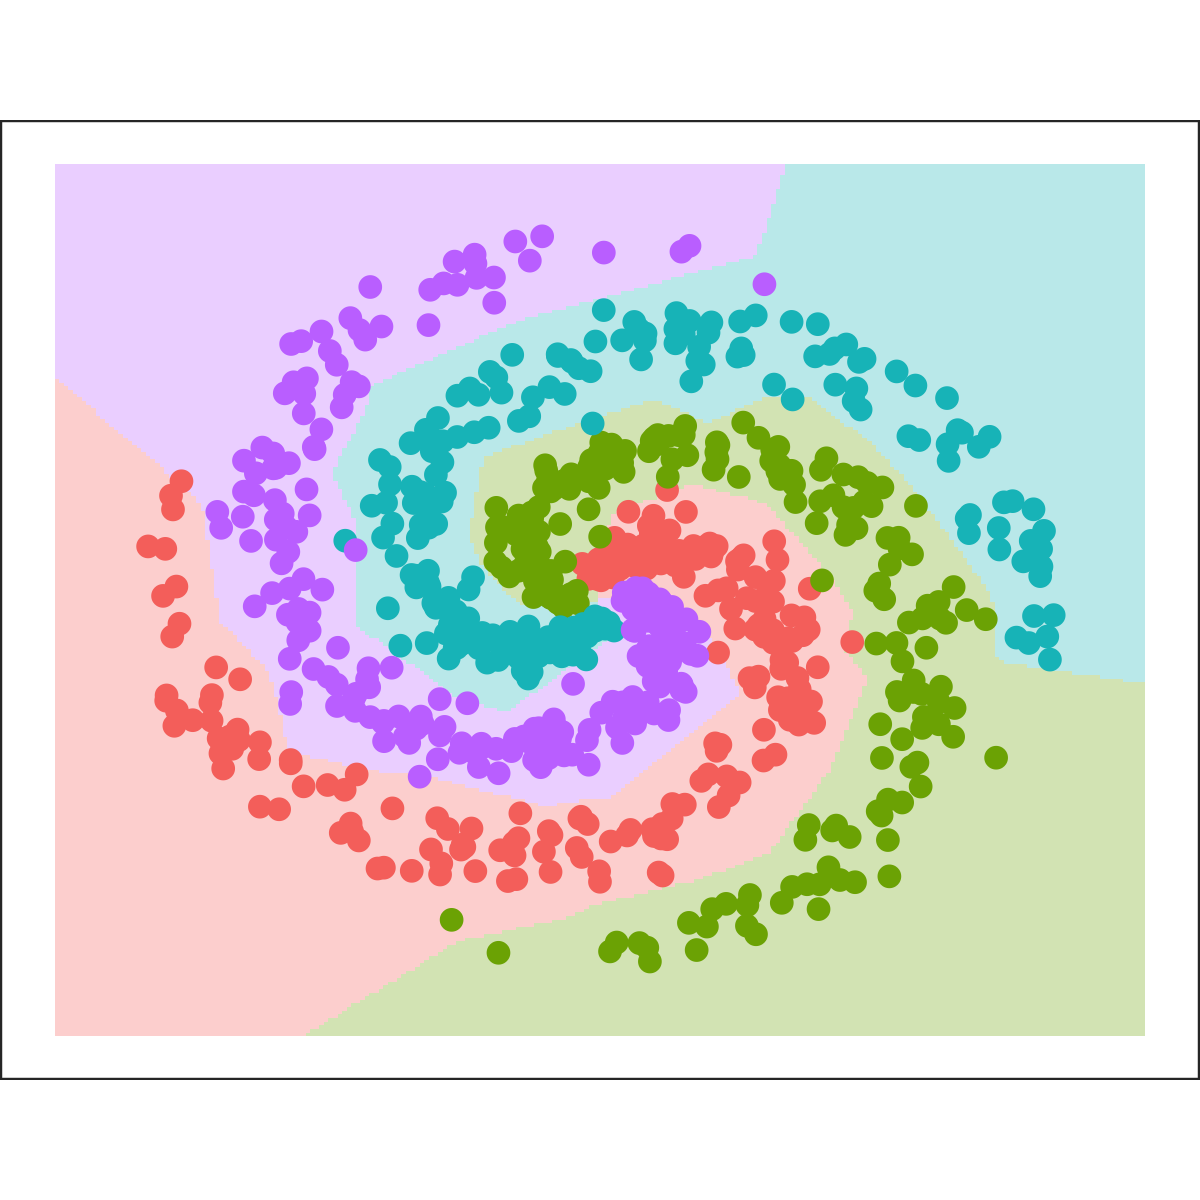
\includegraphics[width=0.9\textwidth]{figures/spiral2.png}
\end{minipage}
\caption{Spiral dataset with 4 different classes.  The shaded region represents the neural network's predictions.}
\end{figure}


% Source: http://junma5.weebly.com/data-blog/build-your-own-neural-network-classifier-in-r

\end{frame}
%%%%%%%%%%%%%%%%%%%%%%%%%%


%%%%%%%%%%%%%%%%%%%%%%%%%%
\begin{frame}
\frametitle{Deep Learning}

\href{https://en.wikipedia.org/wiki/Deep_learning}{\emph{Deep Learning}} employs multiple levels (hierarchy) of representations.

\begin{figure}[!h]
\begin{center}
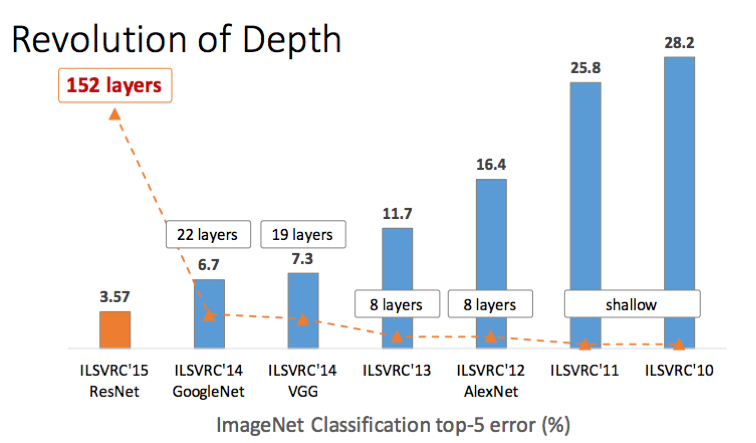
\includegraphics[width=0.95\textwidth]{figures/revo_in_depth.png}
\end{center}
\end{figure}

%https://medium.com/@Lidinwise/the-revolution-of-depth-facf174924f5#.66gerjcg5
%http://torch.ch/blog/2016/02/04/resnets.html
%http://playground.tensorflow.org/#activation=tanh&regularization=L1&batchSize=10&dataset=circle&regDataset=reg-plane&learningRate=0.03&regularizationRate=0.01&noise=20&networkShape=5,2,2&seed=0.62288&showTestData=false&discretize=false&percTrainData=50&x=true&y=true&xTimesY=false&xSquared=false&ySquared=false&cosX=false&sinX=false&cosY=false&sinY=false&collectStats=false&problem=regression&initZero=false&hideText=false

\end{frame}
% %%%%%%%%%%%%%%%%%%%%%%%%%%
% \frame{\frametitle{Convolution Networks}
% 
% Deep neural networks typically have an architucture of major components.
% 
% \begin{figure}[!h]
% \begin{center}
% 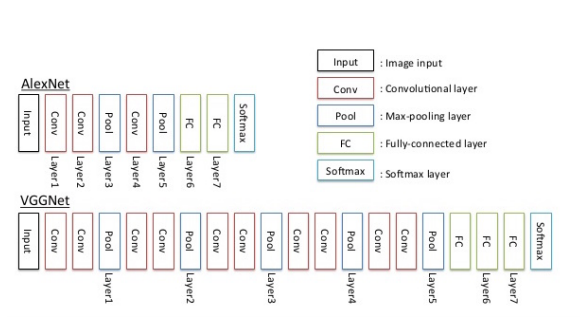
\includegraphics[width=0.95\textwidth]{figures/deep_networks.png}
% \end{center}
% \end{figure}
% 
% }


\begin{frame}

\begin{figure}[!h]
\begin{center}
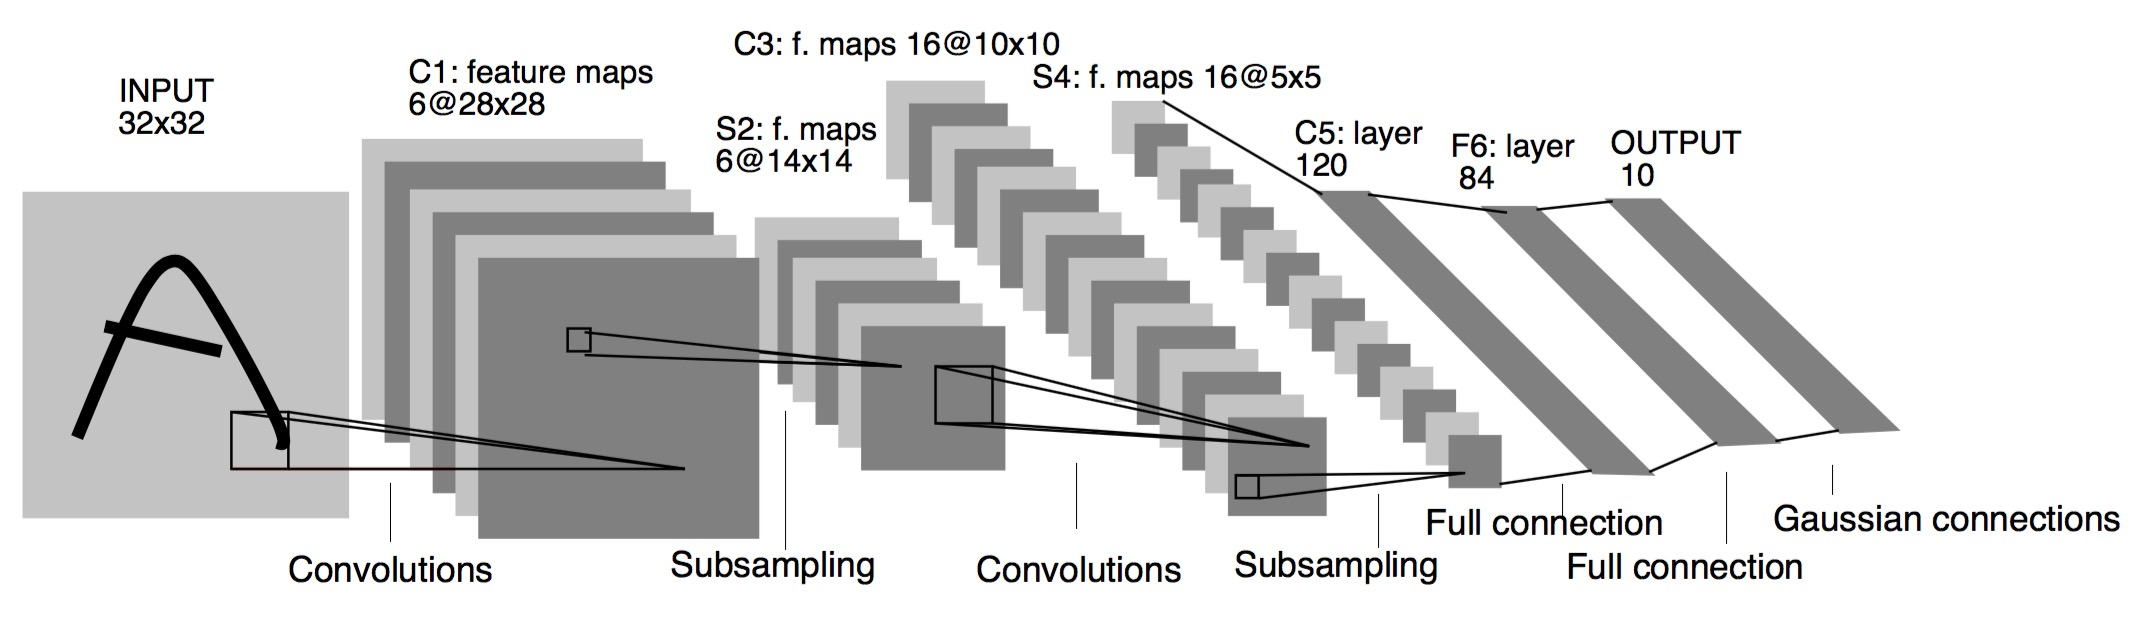
\includegraphics[width=0.8\textwidth]{figures/lenet5.jpg}
\caption{LeNET (1998), Yann LeCun et. al.}
\par\vfill
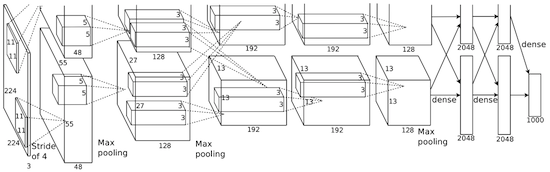
\includegraphics[width=0.8\textwidth]{figures/alexnet_small.png}
\caption{AlexNET (2012), Alex Krizhevsky, Ilya Sutskever and Geoff Hinton}
\end{center}
%\caption{Titanic data from Kaggle competition shows a pattern predicting who survived: more likely to be female, wealthy, and/or young.  Can we model this?}
\end{figure}

\tiny{\emph{Source: \href{http://cs231n.github.io/convolutional-networks/}{Andrej Karpathy}}}

%https://arxiv.org/pdf/1605.07678.pdf

\end{frame}


%%%%%%%%%%%%%%%%%%%%%%%%%%
\begin{frame}
\frametitle{Hierarchical levels of abstraction} 

\begin{figure}[!h]
\begin{center}
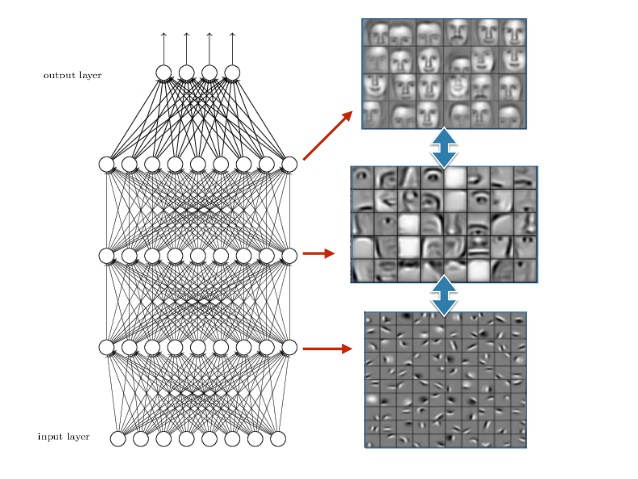
\includegraphics[width=0.8\textwidth]{figures/layers.jpg}
\end{center}
\end{figure}

%http://cs231n.github.io/convolutional-networks/
%https://beckmw.wordpress.com/2013/11/14/visualizing-neural-networks-in-r-update/

\end{frame}



\section{Deep Reinforcement Learning} 

{
\usebackgroundtemplate{% width=\paperwidth,
\parbox[c][\paperheight][c]{\paperwidth}{
\begin{figure}[H]
\begin{center}
%   \tikz\node[opacity=0.2] {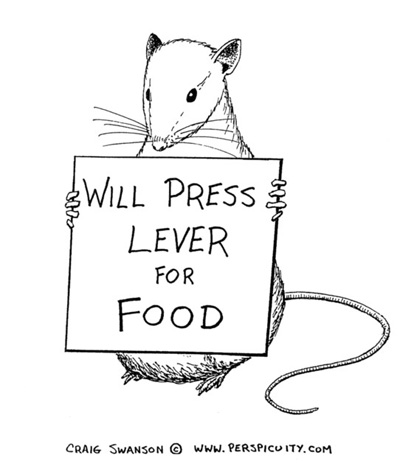
\includegraphics[height=\paperheight, right]{../images/cartoon_4.jpg}};
\end{center}
\end{figure}
}
}

\frame{

\begin{center}
{\huge Deep Reinforcement Learning}\\

\vspace{12 mm}

{\Large Learning how to act on our model of the world.}
\end{center}

}
}

\frame{\frametitle{Reinforcement Learning} 

In a single agent version, we consider two major components: the \emph{agent} and the \emph{environment}.  

\begin{figure}[H]
\begin{center}
\begin{tikzpicture}[->,>=stealth',shorten >=1pt,auto,node distance=2cm,
  thick,main
  node/.style={circle,fill=myblue,draw,text=white,font=\sffamily\Large\bfseries}]
 %nodes
 \node[] (center);
 % We make a dummy figure to make everything look nice.
 \node[top=of center, fill=myblue, text=white] (t) {Agent};
 \node[below=of center, fill=myblue, text=white] (g) {Environment};

  \path[every node/.style={font=\sffamily\small}]
  (t) edge[bend left=65] node[auto] {Action} (g)
  (g) edge[bend left=65] node[auto] {Reward, State} (t);
\end{tikzpicture}
\end{center}
% \caption[Generalized Policy Iteration]
%  {The reinforcement learning cycle, from agent to environment, back to agent.}
  \label{fig:reinforcement_cycle}
\end{figure}

The agent takes actions, and receives updates in the form of state/reward pairs.

\note{
The environment is the real world, which gives the agent some form of feedback.  We can think of the environment as being $y$ and the agent as having $f(x)$, an estimate of the true $y$.
}

}


\frame{\frametitle{Policy} 

The objective is to find a policy $\pi$ that maps actions to states, and will maximize the rewards over time:

{\huge
\begin{center}
\begin{equation*}
\pi(s) \rightarrow a
\end{equation*}
\end{center}
}

\vspace{0.25in}

The policy can be a table or a model (in DeepRL, the model will be a deep neural network).

% \begin{beamerboxesrounded}[shadow=true]{Policy}
% \end{beamerboxesrounded}

}



\frame{\frametitle{DQN} 

DeepMind introduced Deep Q-Networks (DQN) for generally solving Atari games from pixels.  

\begin{figure}[!h]
\begin{center}
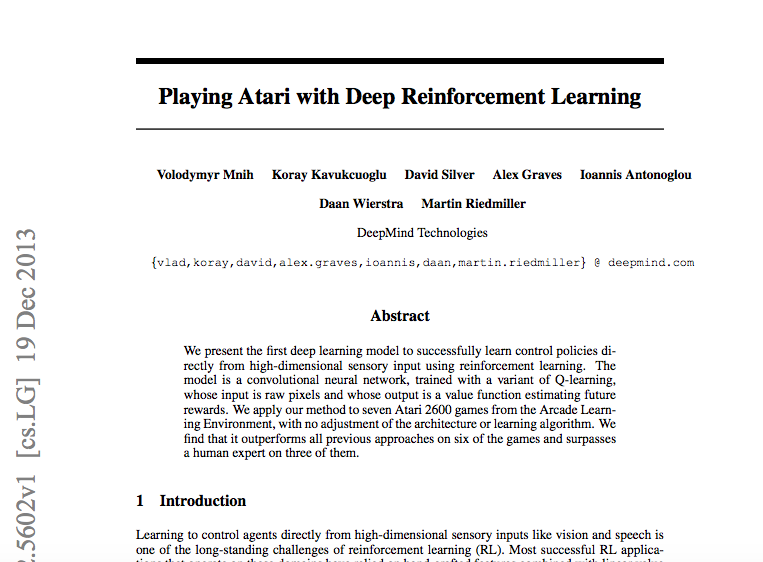
\includegraphics[width=0.75\textwidth]{figures/dqn_paper.png}
\end{center}
\end{figure}


%\vspace{0.15in}

%\scriptsize{\textit{\href{http://neuro.cs.ut.ee/demystifying-deep-reinforcement-learning/}{Source code from DeepMind}}}
 
}


\frame{\frametitle{DQN Network} 

\begin{figure}[!h]
\begin{center}
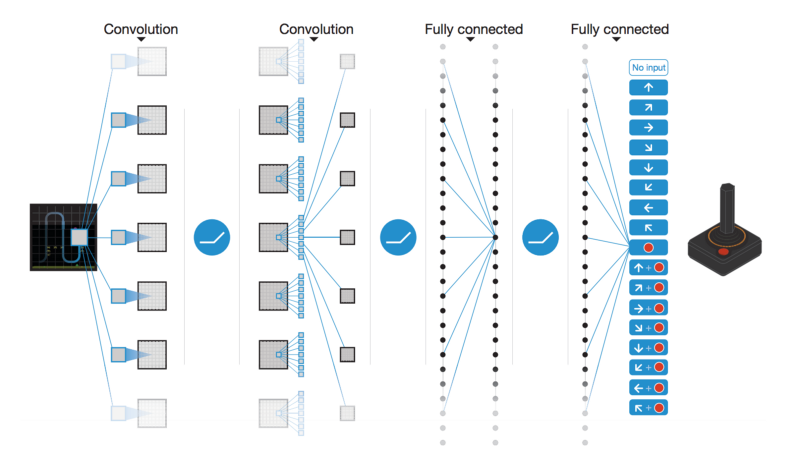
\includegraphics[width=0.95\textwidth]{figures/dqn_network.png}
\end{center}
\end{figure}

\vspace{0.15in}

\scriptsize{\textit{\href{https://sites.google.com/a/deepmind.com/dqn/}{Source code from DeepMind}}}

%https://deepmind.com/research/open-source/open-source-code/ 

}



\frame{\frametitle{Policy network} 

\begin{figure}[!h]
\begin{center}
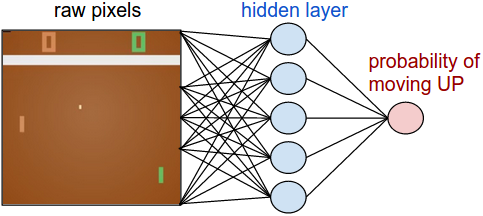
\includegraphics[width=0.9\textwidth]{figures/pong_policy.png}
\end{center}
\end{figure}

\vspace{0.25in}

\scriptsize{\textit{\href{http://karpathy.github.io/2016/05/31/rl/}{Source: @karpathy}}}

}


\frame{\frametitle{Network Weights} 

\begin{figure}[!h]
\begin{center}
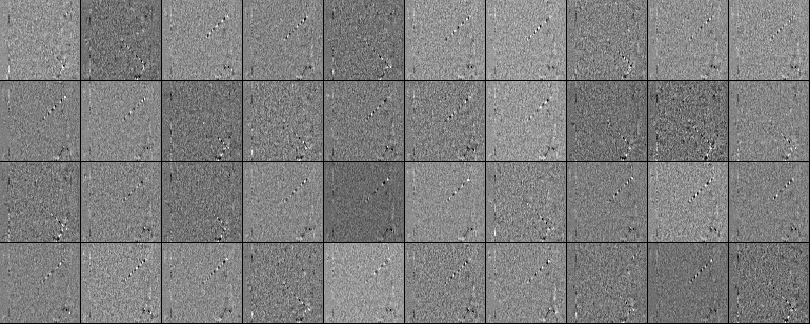
\includegraphics[width=0.95\textwidth]{figures/pong_weights.png}
\end{center}
\end{figure}

\vspace{0.25in}

\scriptsize{\textit{\href{http://karpathy.github.io/2016/05/31/rl/}{Source: @karpathy}}}

}


\begin{frame}
\frametitle{AlphaGo}

AlphaGo combined supervised learning and reinforcement learning, and made massive improvement through self-play.

\begin{figure}[!h]
\begin{center}
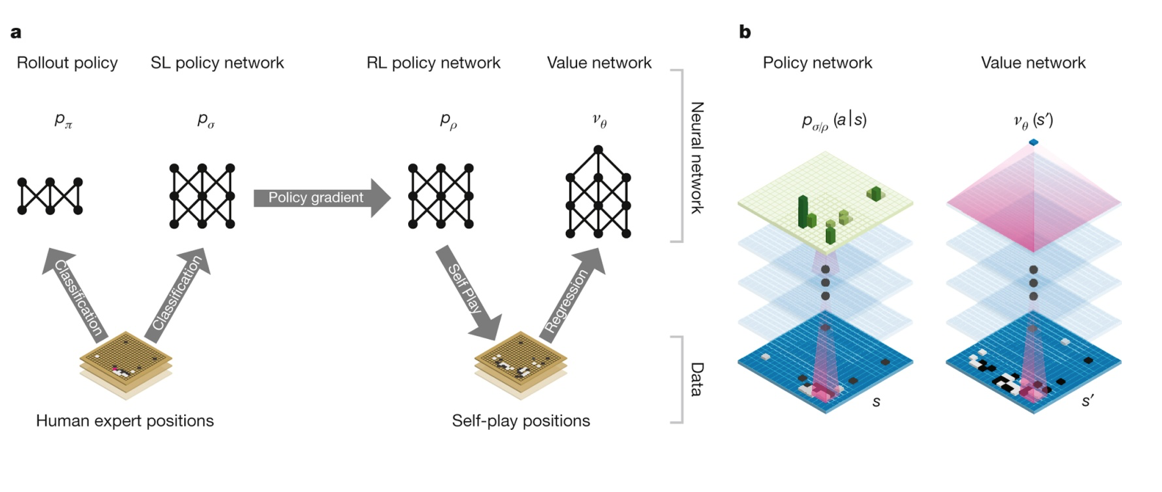
\includegraphics[width=0.9\textwidth]{figures/alphago_network.png}
\end{center}
\end{figure}

%http://deeplearningskysthelimit.blogspot.com/2016/04/part-2-alphago-under-magnifying-glass.html
%https://www.tastehit.com/blog/google-deepmind-alphago-how-it-works/

\end{frame}


\frame{

\begin{center}
{\huge Thank you!}\\
\end{center}

}

\end{document}

